\chapter{Visualisatieframework voor Unipept} 
\chaptermark{Visualisatieframework}
\label{chap:vis}

In dit hoofdstuk schetsen we eerst kort het overzicht van de huidige
visualisaties in Unipept. We staan stil bij de nood aan en het praktisch nut van
het abstraheren van die visualisaties in een apart framework en de voordelen
hiervan. Daarna kijken we naar de implementatie van deze abstractie, waarbij we
de abstractie van de \texttt{treeview}-visualisatie als voorbeeld uitwerken.
Vervolgens gaan we verder in op enkele voorbeelden, use cases en optimalisaties
van de \texttt{treeview}-visualisatie.

\section{Overzicht van visualisaties in Unipept}
\sectionmark{Overzicht}

\label{sec:unipeptvis} 

Vooraleer we overgaan tot de bespreking van het visualisatieframework kijken we
eerst welke visualisaties in Unipept verwerkt zijn. De eerste visualisatie die
we bespreken is de \texttt{treeview}. Deze visualisatie geeft bij een tryptische
peptidenanalyse een overzicht van de taxonomische portie van alle Uniprot
records waarin een bepaalde peptide wordt gevonden en mapt deze voorkomens
vervolgens op een boomstructuur. Een voorbeeld hiervan is te vinden in
\Cref{fig:overzicht1} op \cpageref{fig:overzicht1} De
\texttt{treeview}-visualisatie wordt ook gebruikt binnen de metaproteomics
analyse. Gegeven een lijst van peptides uit een staal, wordt voor elke peptide
de lowest common ancestor berekend. Vervolgens worden de lowest common ancestors
gemapt op de boomstructuur.

\begin{figure}
    \centering
    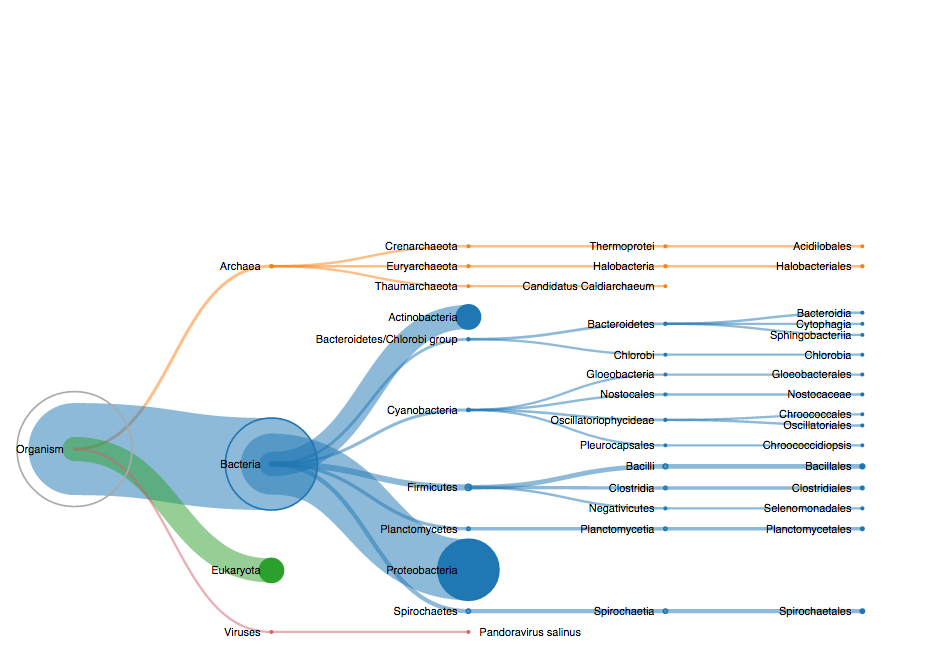
\includegraphics[width=1\textwidth]{includes/visoverzicht1}
    \caption{Voorbeeld van de \texttt{treeview}-visualisatie voor het weergeven 
    van de taxonomische porties van alle UniprotKB eiwitten die de tryptische 
    peptide ``AALTER'' bevatten.}
    \label{fig:overzicht1}
\end{figure}

Er zijn ook twee alternatieve visualisaties voor de tryptische peptidenanalyse.
Het eerste alternatief is een \texttt{sunburst}-diagram, te zien in
\Cref{fig:overzicht2} op \cpageref{fig:overzicht2}. In deze visualisatie zien we
in het centrum de \texttt{root}-taxon. Rond om rond deze centrumnode bevinden
zich de kinderen van het \texttt{root}-taxon. Het is mogelijk om op een kind te
klikken, zodat dat kind het nieuwe centrum van het diagram wordt. Door op de
centrumnode te klikken wordt er een niveau uitgezoomed. Het tweede alternatief
is de \texttt{treemap}-visualisatie. Dit is een 2D weergave van alle gevonden
taxons in de analyse, waarbij de grootte van hun vlak overeenstemt met het
aantal peptidesequenties die specifiek zijn tot op dat niveau. Door op een vlak
te klikken kunnen we inzoomen. Deze visualisatie is te zien op
\Cref{fig:overzicht3}.

Ook bij de de peptidom analyse worden twee visualisaties gebruikt. Bij een 
peptidome analysis worden verschillende volledig gesequeneerde
genomen met elkaar vergeleken. Uit deze analyses worden zaken afgeleid zoals
de grootte van het aantal peptides binnen de core, pan of unique peptidome, of
hoe goed verschillende genomen met elkaar clusteren. De eerste van deze twee die
de groottes van de verschillende peptidomes aangeeft is de
\texttt{pancore}-grafiek. Een voorbeeld hiervan is te zien in
\Cref{fig:overzicht4} op \cpageref{fig:overzicht4}. De clusteringsanalyse
gebeurt aan de hand van een similariteitsmatrix waarbij donkere kleuren een
grotere similariteit tussen twee genomen aanduiden, ondersteund door een
klassieke phylogenetische boom. Een voorbeeld hiervan kan geraadpleegd worden in
\Cref{fig:overzicht5} op \cpageref{fig:overzicht5}.


\begin{figure}
    \centering
    \begin{subfigure}{0.45\textwidth}
        \centering
        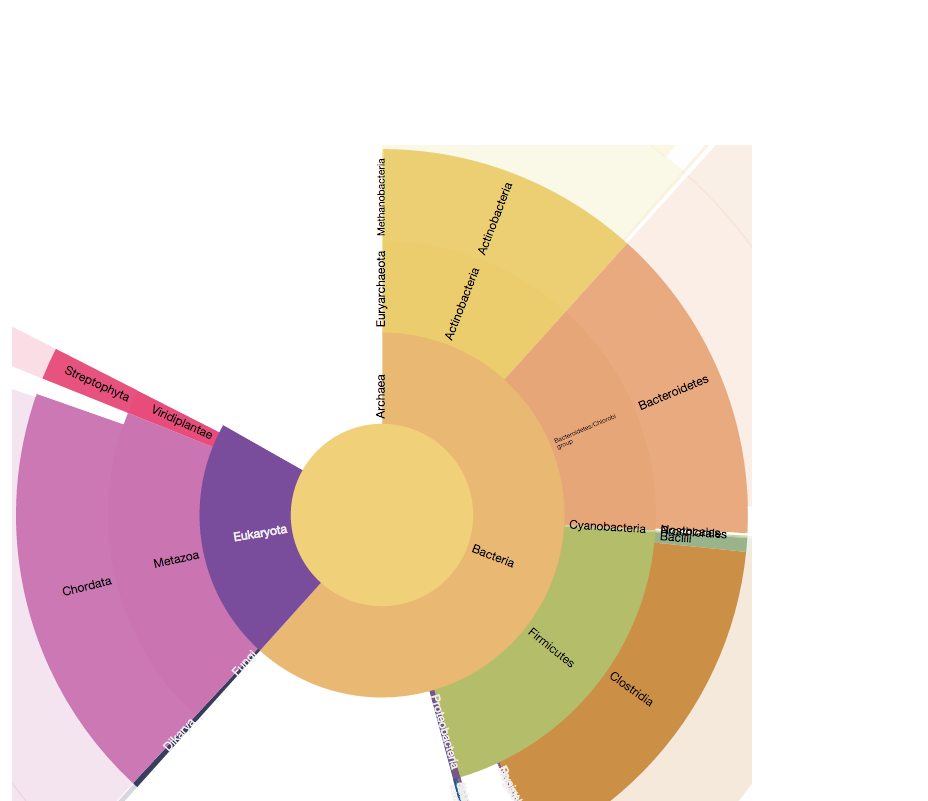
\includegraphics[width=\textwidth]{includes/visoverzicht2}
        \caption{}
        \label{fig:overzicht2}
    \end{subfigure}
    \begin{subfigure}{0.45\textwidth}
        \centering
        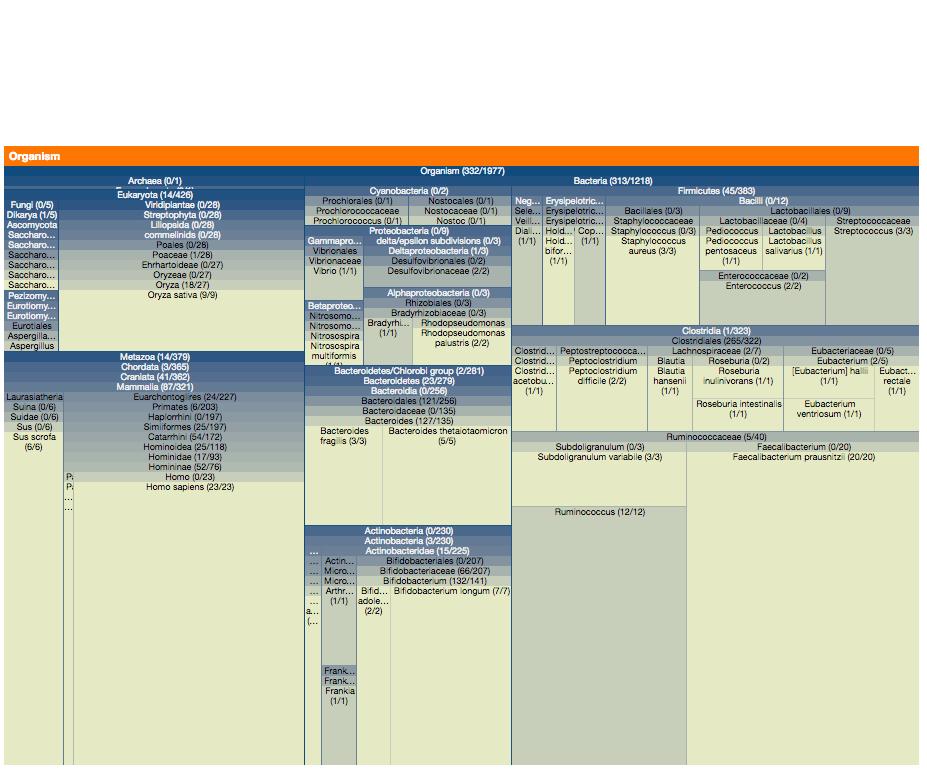
\includegraphics[width=\textwidth]{includes/visoverzicht3}
        \caption{}
        \label{fig:overzicht3}
    \end{subfigure}
    
    \begin{subfigure}{0.45\textwidth}
        \centering
        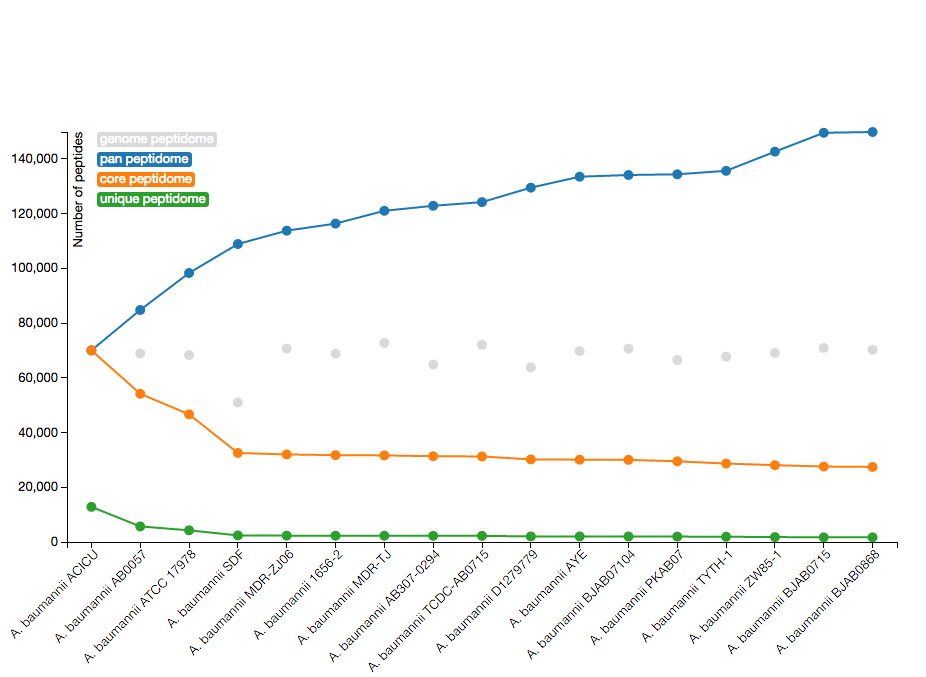
\includegraphics[width=\textwidth]{includes/visoverzicht4}
        \caption{}
        \label{fig:overzicht4}
    \end{subfigure}
    \begin{subfigure}{0.45\textwidth}
        \centering
        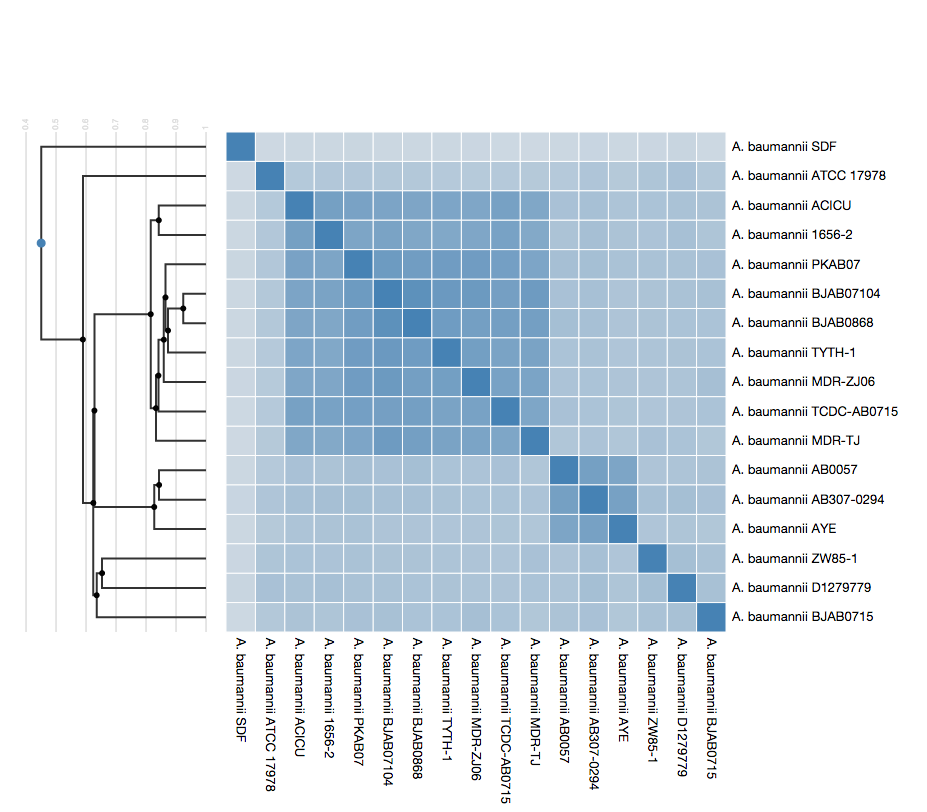
\includegraphics[width=\textwidth]{includes/visoverzicht5}
        \caption{}
        \label{fig:overzicht5}
    \end{subfigure}
    \caption{Overzicht van de visualisaties in Unipept. Linksboven zien we een 
    \texttt{Sunburst}-voorbeeld van een analyse van de metaproteomics dataset 
    van het ``human gut'', met daar rechts van de \texttt{treemap} voor 
    dezelfde dataset. Linksonder wordt een \texttt{pancore} visualisatie 
    getoond van het peptidome van \textit{Acinetobacter Baumannii} met rechts 
    de similariteitsmatrix met bijhorende phylogenetische boom voor hetzelfde 
    organisme.}
    \label{fig:overzicht}
\end{figure}

Alle visualisaties zijn geschreven met behulp van D3. D3 is een JavaScript
bibliotheek voor het maken van een dynamische en
interactieve visualisaties aan de hand van HTML, CSS en SVG\cite{D3.js6:online}.

\section{Modularisatie en abstractie} 
\label{sec:modenabs} 

Momenteel zitten alle visualisaties volledig verankerd in Unipept en zijn ze
zeer dicht verweven met de Unipept webinterface. Deze integratie brengt enkele
voordelen met zich mee. Zo kan de code bijvoorbeeld eenduidig en specifiek
geschreven worden voor één gewenst doel, zonder rekening te moeten houden met
eventuele mogelijkheden die toch niet zullen voorkomen of zouden gewenst zijn.
Volledige integratie heeft echter ook zijn nadelen. Zo is het niet mogelijk
dezelfde visualisatie in een andere omgeving of voor een ander doel te
gebruiken, zonder de achterliggende code aan te passen. Met de huidige
implementatie kunnen er bijvoorbeeld geen twee treeviews naast elkaar 
weergegeven worden, kan er niet gemakkelijk andere data (zoals niet-biologische 
data) aan de boom gekoppeld worden, enzovoort.

Binnen de context van deze thesis wordt de treeview als een overzichtelijke
visualisatie gebruikt om (delen van) de volledige NCBI taxonomie weer te geven.
We gebruiken de treeview als visueel hulpmiddel om onder andere het effect van
invalidaties van taxons op de treeview te visualiseren of om het effect van in
\Cref{sec:lca*} beschreven analyses weer te geven. Om dit te verwezenlijken moet
het mogelijk zijn op een eenvoudige manier willekeurige data in te voeren en
moeten de visualisatieopties snel kunnen ingesteld worden, zonder daarbij steeds
de achterliggende code te moeten aanpassen. Daarnaast willen we ook meerdere
treeviews op één pagina visualiseren, zodat niet telkens van scherm moet
gewisseld worden bij het vergelijken van twee resultaten. Kort gesteld willen we
vertrekken van een bepaald invoerformaat, om zo snel mogelijk een gevisualiseerd
resultaat te zien krijgen, zonder de invoer in een webinterface in te geven.

In de informatica heet dit concept ``modularisatie'': stukken code worden
onderverdeeld in afgesloten modules waarbinnen ze apart worden ontwikkeld en
onderhouden. De aparte modules kunnen vervolgens samen ingeplugd worden in een
groter systeem. Door abstracties toe te voegen kunnen aparte modules niet enkel
voor één doel gebruikt worden, maar kunnen ze ook dienst doen in andere
projecten die niet per sé het visualiseren van data uit de metaproteomics als
doel hebben.

Zoals eerder vermeld zijn de huidige visualisaties enkel beschikbaar binnen de
Unipept webinterface. Dit werkt goed bij kleine hoeveelheden data, maar wanneer
we grote datasets willen inladen, duiken er problemen op en weigert de browser.
We kunnen dit probleem oplossen door de visualisaties los te koppelen van de
codebase van het huidige Unipept platform en door ze als zelfstandige modules
aan te bieden. In combinatie met de bestaande command line tools kunnen we dan
de visualisatiemodule gebruiken om de resultaten visueel weer te
geven door de data via een webinterface in te laden en te verwerken.

Het modulariseren van die visualisaties kan dus een stap in de goede richting
zijn om ze ook buiten de Unipept webinterface aan te bieden. Als we kijken naar
de huidige staat van visualisaties buiten Unipept, moeten we vaststellen dat die
niet optimaal is. Vaak zijn de visualisaties statisch en proberen ze te veel
data in één opzicht weer te geven, wat het resultaat complex en onoverzichtelijk
maakt. Het aanbieden van een open-source en een geabstraheerd
visualisatieframework zou hier een oplossing voor kunnen bieden.

Dit is een argument voor modularisatie, maar ook abstractie speelt een rol.
Zonder het toevoegen van abstractie kunnen de huidige visualisaties enkel
gebruikt worden om één soort data voor te stellen, wat altijd in exact dezelfde
visualisatie resulteert. Door het toevoegen van abstractie krijgt de gebruiker
de mogelijkheid om de voorstelling van de boom eenvoudig te wijzigen, zonder
daarbij aanpassingen in de onderliggende broncode te moeten maken.

\section{Implementatie}

De concepten van modularisatie en abstractie liggen dicht
bij elkaar. Door iets modulair te maken, maak je het vanzelf abstracter. In 
deze sectie kijken we eerst hoe andere JavaScript frameworks dit
realiseren. Daarna bespreken we de implementatie hiervan aan de
hand van een hands-on voorbeeld van de treeview-visualisatie.

\subsection{Modularisatie}
Bootstrap\cite{Boots1:online} is waarschijnlijk het meest bekende
Javascriptframework. Bootstrap biedt een hele reeks JavaScriptbibliotheken aan
om bepaalde ontwerppatronen op het web eenvoudiger te kunnen implementeren.
Gebruikers kunnen alle functies samen in één pakket downloaden maar hebben ook
de mogelijkheid om één functie te selecteren en enkel die te gebruiken.
Aangezien de functionaliteiten van Bootstrap alleen, gedeeltelijk of volledig
ingeplugd kunnen worden als modules, doet Bootstrap duidelijk aan modularisatie.

\subsubsection{Case study: Bootstrap Carousel}

Als we de code van Bootstrap in detail bekijken, zien we dat alle Bootstrap 
plugins eenzelfde coderichtlijn gebruiken. \autoref{lst:bootstrapcarousel} op  
\autopageref{lst:bootstrapcarousel} laat een (ingekort) voorbeeld 
zien van de Bootstrap \texttt{Carousel}-klasse.\cite{bootscarrousel:online}. 
Eerst wordt een
constructor\footnote{Gebruik van OOP terminologie in JavaScript staat ter
discussie, maar maakt het redeneren over de structuur eenvoudiger. Vanaf
ECMAScript 6 zijn ook OOP keywords in JavaScript beschikbaar.} gedefinieerd om 
een
\texttt{Carousel} aan te maken, waarna enkele standaardwaarden worden toegekend
aan de klasse \texttt{Carousel} om de versie en andere standaardwaarden in te
stellen. Daarna worden enkele methodes op de klasse gedefinieerd die toelaten
om de staat van een object aan te passen.

Als we de functie \texttt{Plugin} tijdelijk overslaan zien we iets merkwaardigs.
De functie \texttt{carousel} wordt gelijk gesteld aan een call naar de functie
\texttt{Plugin} door middel van de lijn \lstinline|$.fn.carousel = Plugin|. Dat
wil zeggen dat we aan het \texttt{\$} object -- waarbij \texttt{\$} een
afkorting is van jQuery -- een methode genaamd \texttt{carousel} toevoegen,
waarbij oproepen in de vorm van \lstinline|jQueryObject.carousel()| terechtkomen
bij de methode \texttt{Plugin}.

Zo kunnen we bijvoorbeeld in een HTML-bestand een \texttt{div} maken, de
\texttt{div} selecteren aan de hand van zijn \texttt{id} of \texttt{class}, en
daarna de functie \texttt{carousel()} aanroepen. Op dit \texttt{div} object zal
dan de functie \texttt{Plugin} worden aangeroepen.

Ook de lijn \lstinline|$fn.carousel.Constructor = Carousel| heeft wat meer
uitleg nodig. Het toekennen van een klasse aan het
\texttt{Constructor}-attribuut van een plugin zorgt ervoor dat de constructor
van buitenaf toegankelijk is. Zo kan een programmeur bijvoorbeeld rechtstreeks
een \texttt{Carousel} definiëren door middel van 
\texttt{var myCarousel = new \$.fn.carousel.Constructor()} zonder gebruik te 
maken van de \texttt{Plugin}
methode. De naamgeving van het \texttt{Constructor} attribuut is puur conventie.

Tot nu toe was alle code relatief rechtoe rechtaan. De echte ``magie'' om de
\texttt{Carousel}-klasse modulair inplugbaar te maken, vindt plaats in de
\texttt{Plugin} methode. In de eerste lijn van deze functie overlopen we via
\lstinline|this.each()| alle jQuery elementen waarop de methode -- in dit geval
-- \texttt{carousel} is opgeroepen. Om ervoor te zorgen dat we verdere methodes
kunnen schakelen aan de oproepende methode geven we de DOM-elementen ook
terug\cite{jQueryChaining:online}.

Op elk DOM-element roepen we een anonieme functie op waarbij de \texttt{this}
variabele (die een DOM element voorstelt) omvormen tot een jQuery object zodat
jQuerymethodes hier op kunnen worden opgeroepen. In de variabele \texttt{data}
wordt opgeslagen of er reeds een data-attribuut is toegekend. Daarna stellen we
een lijst op van opties via de jQuery \texttt{extend}-methode. Hierbij worden
drie opties gemengd. i) de defaultwaarden van de \texttt{Carousel}-klasse, ii)
eventuele attributen die meegegeven worden via data-attributen aan het
DOM-element en iii) opties die worden meegegeven via de parameters van de
\texttt{carousel}-functie.

Als de \texttt{data}-variabele nog niet ingesteld werd, stellen we die nu in. 
Om dat
te doen zetten we het data-attribuut van het huidig DOM-element op
\texttt{bs.carousel}, en maken we een nieuwe instantie van de
\texttt{Carousel}-klasse met de gemende opties uit de vorige paragraaf. Het
data-attribuut van het betreffende DOM-element geeft nu aan of er al een
carousel is geïnitialiseerd of niet. Als we de \texttt{carousel}-functie
oproepen op een DOM-element waar reeds een \texttt{carousel} is geïnitialiseerd,
kunnen we afhankelijk van het type van de parameters verschillende acties
uitvoeren op de het DOM-element, die dan de reeds geïnitialiseerde carousel
bevat.

\begin{lstlisting}[caption=Ingekorte Bootstrap code van de 
\texttt{Carousel}-plugin, 
label=lst:bootstrapcarousel]
// Creatie van de klasse Carousel
var Carousel = function (element, options) {
  this.$element    = $(element)
  this.options     = options
  this.paused      = null
  // Andere klassevariabelen kunnen hier worden gedeclareerd
  ...
}

// Declaratie van globale variabelen
Carousel.VERSION  = '3.3.4'
Carousel.TRANSITION_DURATION = 600
Carousel.DEFAULTS = {
interval: 5000,
  ...
}

// Methoden kunnen worden toegevoegd via het prototype van het Carousel object
Carousel.prototype.some_method = function (params) {
  ...
}

// Toevoegen van de gemaakte klasses en methoden aan het jQuery object
$.fn.carousel             = Plugin
$.fn.carousel.Constructor = Carousel

// Methode die bovenstaande Carousel klasse modulair inplugbaar maakt
function Plugin(option) {
  return this.each(function () {
    var $this   = $(this)
    var data    = $this.data('bs.carousel')
    var options = $.extend(
      {}, 
      Carousel.DEFAULTS, 
      $this.data(), 
      typeof option  == 'object' && option
    )

    /* Initialiseert een nieuwe carousel wanneer $this geen data-
    attribuut heeft met de waarde `bs.carousel`. */
    if (!data) $this.data('bs.carousel', (data = new Carousel(this, options)))
    // Voer methodes uit afhankelijk van de argumenten
    if (typeof option === 'number') data.to(option)
    else if ...
  })
}
\end{lstlisting}

Kort samengevat: Bootstrap gebruikt een objectgeoriënteerde structuur waar,
afhankelijk van het bestaan van een bepaald data-attribuut, een nieuwe instantie
van een bepaalde klasse aan een jQuery element wordt gehangen of waar methodes
worden aangeroepen op een reeds bestaande instantie. Het koppelen van instanties
van een klasse aan een jQuery element is daarbij de motor om alles modulair te
maken. Op die manier kan aan gelijk welk DOM-element een Bootstrapcomponent
gehangen worden, zonder dat de interne code de naam of id van dit object moet
kennen.

\subsubsection{Huidige Treeview implementatie in Unipept}

Bootstrap gebruikt hier dus een strategie die een oplossing biedt voor de
tekortkomingen van de \texttt{treeview}-visualisatie. Een gemodereerd deel van
de oorspronkelijke code is te zien in \autoref{lst:unipepttreeview} op
\autopageref{lst:unipepttreeview}. Hierbij wordt alle code omvat in één functie,
\texttt{constructTreeview}. Bij een oproep van die functie wordt de binnenste
\texttt{init}-functie opgeroepen die enkele zaken initialiseert. De functie
bindt eerst de \texttt{reset}-functie aan een knop met id
\texttt{treeview-reset}, waarna de functie de benodigde functies oproept om de
treeview ook werkelijk te tekenen, zijnde \texttt{redraw}- en \texttt{draw}.
Onderaan wordt ook de methode \texttt{reset} publiek beschikbaar gemaakt door
deze (en eventueel andere publieke methodes) te binden aan de \texttt{that}
variabele. Het \texttt{that} object wordt op het einde van de omvattende functie
teruggegeven, zodat de publieke functies via het object kunnen opgeroepen
worden.

De methode \texttt{constructTreeview} kan zo door een gebruiker opgeroepen
worden, waarbij de gebruiker het resultaat (het \texttt{Treeview}-object) kan
opslaan om methodes op dit object op te roepen.

\begin{lstlisting}[caption=Gemodereerde TreeView code, 
label=lst:unipepttreeview]
/**
 * Maakt een Treeview object die de visualisatie representeert
 */
var constructTreeview = function constructTreeview(args) {
    /*************** Private variabelen ***************/

    // parameters
    var that = {},
        multi = args.multi,
        data = args.data;

    // private variabelen
    var privateVariable = name;

    /*************** Private methoden ***************/

    // Initialiseert een Treeview
    function init() {
        // init controls
        initControls();

        // draw everything
        redraw();
        draw(data);
        
        ...
    }

    // Initieert controllers
    function initControls() {
        // bindt de reset-methode aan het #treeview-reset element
        $("#treeview-reset").click(that.reset);
    }

    // Hertekent de treeview
    function redraw() {
        // Maak de treeivew leeg
        $("#d3TreeView").empty();
        
        ...
        
        // Tekent de d3 visualisatie op het #d3TreeView element
        svg = d3.select("#d3TreeView").append("svg")
        
        ...
    }
    
    // Tekent de boom
    function draw(data) { ... }

    /*************** Publieke methoden  ***************/

     // Zet de visualisatie in zijn oorspronkelijke staat terug
    that.reset = function reset() {
        zoomListener.scale(1);
        rightClick(root);
    };

    // initaliseert het object
    init();

    // geef het object terug
    return that;
};
\end{lstlisting}

De code die net werd beschreven functioneert goed wanneer die enkel binnen
Unipept gebruikt wordt, maar is zeker niet modulair genoeg om als framework aan
te bieden. Het grootste verschil tussen de twee benaderingen is het binden van
de visualisatie aan een DOM-element. Bij een Bootstrap plugin gebeurt dit door
een methode (in voorgaand voorbeeld \texttt{carousel}) op te roepen op een
jQuery object. Bij de huidige implementatie in Unipept wordt dit element
ingesteld in de code zelf. Methodes worden in Bootstrap plugins rechtstreeks op
het element opgeroepen, zonder dat het Javascript object ergens dient te worden
opgeslagen. De koppeling tussen het element en de plugin/visualisatie die
vasthangt aan dat element gebeurt intern via een \texttt{data}-attribuut. In de
implementatie in Unipept moet hiervoor het JavaScript object zelf bijgehouden 
worden en worden methodes rechtstreeks op dit object opgeroepen.

Praktisch houdt dit in dat er op meerdere plaatsen in de Unipept-visualisatie
verwezen wordt naar een HTML klasse of id. Dit is nadelig als we deze
visualisaties zouden willen aanbieden aan gebruikers buiten Unipept. Wanneer er
bijvoorbeeld een gebruiker twee verschillende bomen onder elkaar zou willen
weergeven, is dit onmogelijk zonder de hele omvattende methode te dupliceren en
de id waaraan de visualisaties worden gekoppeld aan te passen, of door het
visualisatieobject mee te geven als extra parameter aan de
\texttt{constructTreeview} functie. Ook het koppelen van acties zoals binden van
de \texttt{reset}-methode aan meerdere objecten is met deze strategie niet
mogelijk.

Als we de Unipept visualisaties in een extern visualisatieframework willen
aanbieden, is het wenselijk dat de gebruiker de code nooit zelf hoeft aan te
passen, maar die gewoon vanuit zijn eigen JavaScriptcode kan aanroepen. Door de
Bootstrap \texttt{Plugin}-methode toe te passen op de bstaande code en intern
enkele veranderingen door te voeren, kunnen we de interne code volledig
loskoppelen van onderliggende DOM-elementen, zodat de gebruiker deze plugin --
met natuurlijk de nodige documentatie -- als een blackbox kan behandelen zonder
intern aanpassingen te hoeven aan brengen.

\subsubsection{Implementatie}
\label{sec:modenimp}
De herwerkte code na het integreren van de Bootstrap \texttt{Plugin}-functie is
terug te vinden in \autoref{lst:unipepttreeviewplugin} op
\autopageref{lst:unipepttreeviewplugin}. Erg verschillend van een combinatie van
de vorige twee codefragmenten is dit niet. We zien onderaan dat de
\texttt{treeview}-methode wordt gekoppeld aan de \texttt{Plugin}-methode,
analoog met de Bootstrap \texttt{carousel}-functie. In de
\texttt{Plugin}-methode koppelen we een data-attribuut \texttt{vis.treeview} aan
het opgegeven jQuery-object wanneer dit attribuut nog niet is ingevuld. Bij het
aanmaken van een \texttt{TreeView} object geven we naast het DOM-element waarop
de \texttt{treeview}-methode is aangeroepen, ook de standaard opties en
eventuele opgegeven opties mee. In de \texttt{init}-methode van deze
\texttt{TreeView} klasse koppelen we nu de D3 visualisatie aan het opgegeven
DOM-element. Methodes die van buitenaf beschikbaar moeten te zijn, zoals de
\texttt{reset}-methode, worden aan de variabele \texttt{that} toegekend die
uiteindelijk wordt teruggegeven.

\begin{lstlisting}[caption=(Ingekorte) code van de Unipept Treeview plugin,
label=lst:unipepttreeviewplugin]
// Constructor van het TreeView-object
var TreeView = function TreeView(element, options) {
    var that = {};

    // Private methodes
    function init() {
        ...
        
        svg = d3.select(element).append("svg")
            ...
    }
    
    ...
    
    // Publieke methodes
    that.reset = function reset() { ... }
    
    init();
    
    return that;
};

TreeView.DEFAULTS = { ... }

$.fn.treeview = Plugin;
$.fn.treeview.Constructor = TreeView;

// Pluginmethode
function Plugin(option) {
    return this.each(function () {
        var $this = $(this);
        var data = $this.data('vis.treeview');
        var options = $.extend(
            {}, 
            TreeView.DEFAULTS, 
            $this.data(), 
            typeof option === 'object' && option
        );

        if(!data) { 
            $this.data('vis.treeview', 
                       (data = new TreeView(this, options))); 
        }
        if(typeof option === 'string') { data[option](); }
    });   
}
\end{lstlisting}

Dit zorgt ervoor -- net zoals in de Bootstrap Carousel case study -- dat 
er een
treeview-visualisatie kan worden gehangen aan eender welk DOM-element door het
oproepen van de \texttt{treeview}-functie. Eén argument is verplicht, namelijk
het \texttt{data}-argument dat de te visualiseren data bevat. Publieke 
methoden, zoals de \texttt{reset}-methode kunnen worden opgeroepen door de 
methodenaam als \texttt{string} mee te geven aan de \texttt{treeview}-function: 
\lstinline|$('#treeviewDiv').treeview('reset')|. Meer voorbeelden zullen 
worden uitgewerkt in \Cref{sec:voorbeelden} op \cpageref{sec:voorbeelden}.

\subsection{Abstractie}
De huidige visualisaties in Unipept zijn, zoals eerder beschreven, specifiek
gemaakt om data uit de Unipept metaproteomics pipeline grafisch weer te geven.
Als we willen dat gebruikers ook de visualisaties kunnen gebruiken voor andere
soorten data, moeten we de specifieke functies abstraheren. Daarnaast willen we
ook een stuk controle in de handen van de gebruiker leggen. Een gebruiker wil
bijvoorbeeld de kleur van de visualisatie kunnen bepalen, de hoogte en breedte
van de visualisatie veranderen, de grootte van de nodes beïnvloeden, etc. We
moeten er dus voor zorgen dat de gebruiker zelf (extra) methodes kan
implementeren, die de standaardmethodes vervangen.

We maken onderscheid tussen twee vormen van abstractie. Ten eerste moet de
gebruiker via parameters instellingen kunnen overschrijven, zoals bijvoorbeeld
de breedte van de visualisatie, de afstand tussen de nodes, etc. Ten tweede moet
de gebruiker ook functies die inspelen op de data kunnen overschrijven. Het
eerste deel hiervan wordt reeds opgelost door het uitbreiden van de standaard
opties met opties die de gebruiker meegeeft aan de Plugin-methode beschreven in
\Cref{sec:modenimp} op \cpageref{sec:modenimp}. Stel dat de gebruiker de hoogte
en breedte van zijn visualisatie wil opgeven, dan kan hij dit doen door de
functie \texttt{treeview} op een DOM-element op te roepen, waarbij hij naast de
te visualiseren data ook de argumenten \texttt{width} en \texttt{height}
meegeeft. De oproep om een visualisatie van 1400 pixels breed op 800 pixels hoog
te maken met als data een object genaamd ``data'' kan er dan bijvoorbeeld zo
uitzien:

\begin{lstlisting}
$("#d3TreeView").treeview({
    data: data,
    width: 1400,
    height: 800
});
\end{lstlisting}

Functies overschrijven kan echter niet zo eenvoudig. Het verschil met gewone
algemene parameters is dat we bij functies willen dat ze afhankelijk zijn van
een bepaalde invoer, bijvoorbeeld de naam van de visualisatiecomponent in
kwestie. De eenvoudigste oplossing hiervoor is om de te overschrijven functies
als standaardmethodes te implementeren op dezelfde hoogte als waar de standaard
waarden gedefinieerd worden. Zo kunnen we bijvoorbeeld een standaardfunctie
implementeren die de opvulkleur van de nodes in de treeview afhankelijk maakt
van het al dan niet hebben van ``kinderen''. Dit zou bijvoorbeeld als volgt als
standaardmethode kunnen worden geïmplementeerd:

\begin{lstlisting}
TreeView.NODE_FILL_COLOR = function(d) {
    if (d.selected) {
        return d._children ? d.color || "#aaa" : "#fff";
    } else {
        return "#aaa";
    }
};
\end{lstlisting}

Deze standaardfunctie kunnen we nu meegeven als parameter aan het
\texttt{TreeView.DEFAULTS}-object dat onder meer ook de bovenstaande
standaardwaarden bevat via \texttt{nodeFillColor: TreeView.NODE\_FILL\_COLOR}.

Indien een gebruiker een andere functionaliteit wenst dan de
standaardfunctionaliteit, dan kan hij zelf een functie declareren die
bijvoorbeeld altijd rood teruggeeft:

\begin{lstlisting}
// Declaratie van eigen kleurfunctie ter vulling van nodes
var nodeFillColor = function(d) {
    return 'red';
}

// Meegeven van eigen kleurfunctie aan de Treeview-bibliotheek
$("#d3TreeView").treeview({
    data: data,
    nodeFillColor: nodeFillColor
});
\end{lstlisting}

Alle functies die de gebruiker moet kunnen overschrijven of aanpassen,
kunnen op deze manier geïmplementeerd worden.

Niet alleen de uitvoer (het visuele resultaat) moet generiek zijn, maar ook de
invoer. Momenteel is de invoer een JSON-object met vier attributen: \texttt{id},
\texttt{name}, \texttt{data} en \texttt{children}. Deze vaste attributen zijn
ook nodig om dezelfde data in andere visualisaties voor te stellen. Aan het
\texttt{data}-attribuut kunnen elementen worden toegevoegd die specifiek zijn
voor de gewenste visualisatie. In de Unipept-visualisaties wordt bijvoorbeeld
altijd gebruik gemaakt van een \texttt{count}-, \texttt{rank}- en
\texttt{self\_count} attribuut. Deze optionele attributen kunnen dan opgeroepen
worden in de functies die de standaardmethodes vervangen. Aangezien we met
hiërarchische visualisaties werken, moeten ook ``kinderen'' aan ``ouders''
toegevoegd kunnen worden. Dit laatste gebeurt door het toevoegen van een lijst
van JSON-objecten van dezelfde vorm als hierboven geschreven aan het
\texttt{children}-attribuut van zijn ``ouder''.

Aangezien de invoer momenteel al generiek en door middel van het
\texttt{data}-attribuut ook naar wens uitbreidbaar is, kunnen we besluiten dat
de invoer voldoende geabstraheerd is.

\section{Case studies}
\label{sec:voorbeelden}
In deze sectie wordt een overzicht van de huidige mogelijkheden geschetst aan 
de hand van enkele use cases, telkens met de betreffende code en het resultaat. 

\subsection{Modularisatie: vergelijken van resultaten van toolchains}
We beginnen met een eenvoudig voorbeeld van de modularisatie. Stel dat een
gebruiker een metagenomics analyse heeft uitgevoerd, gebruik makend van de
\texttt{pept2lca2lca} toolchain  met de command-line tools, en dit resultaat
visueel wil weergeven. Het resultaat van de analyse is een lijst van taxons, hun
rang en id, gegroepeerd per fasta header. De gebruiker kan daarna via een script
\texttt{tax2tree.py} het resultaat omzetten in een JSON-object dat hij
rechtstreeks kan inpluggen in een visualisatie door middel van het HTML bestand
in \Cref{lst:visexample1} op \cpageref{lst:visexample1}. Deze code kan gewoon in
een lokaal HTML bestand worden ingegeven en geeft als resultaat
\Cref{fig:visexample1}.

\begin{lstlisting}[language=HTML,caption={Voorbeeldcode ter illustratie van 
modularisatie van de \texttt{treeview}-visualisatie},label={lst:visexample1}, 
float]
<html>
  <head>
    <title>Unipept Visualisation Framework</title>

    <!-- Inladen van jQuery, Bootstrap en d3 -->
    ...

    <!-- Inladen Visualisatiemodules -->
    <link href="../assets/stylesheets/tooltip.css" rel="stylesheet">
    <script src="../assets/javascripts/treeview.js"></script>

    <script>
      $(function() {
        // Inladen van het te visualiseren JSON-bestand
        d3.json("../sample-data/pept2lca2lca.json", function(error, data) {
          // Initialisatieaanroep van de treeview-methode
          $("#d3TreeView-pept2lca2lca").treeview({data: data});
        });
        
        // Binden van de reset-actie aan de #treeview-reset knop
        $("#treeview-reset-pept2lca2lca").click(function() {
          $("#d3TreeView-pept2lca2lca").treeview('reset');
        });
      });
    </script>
  </head>
  <body>
  <span class="dir">
    <a class="btn btn-xs btn-default" id="treeview-reset-pept2lca2lca" 
    title="reset 
    visualisation"><i class="glyphicon glyphicon-repeat"></i></a>
  </span>
  <span class="dir text">Scroll to zoom, drag to pan, click a node to 
  expand, right click a node to set as root</span>
  <div id="d3TreeView-pept2lca2lca"></div>
  </body>
</html>
\end{lstlisting}

\begin{figure}
    \centering
    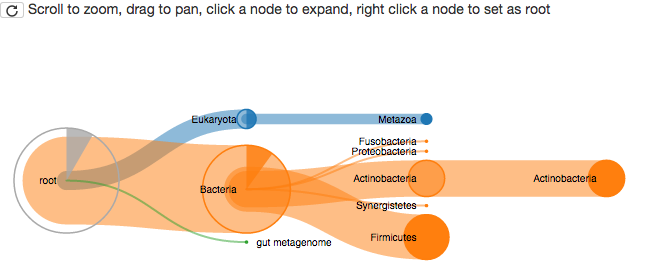
\includegraphics[width=0.9\textwidth]{includes/visexample1}
    \caption{Resultaat van de HTML-code in \Cref{lst:visexample1}}
    \label{fig:visexample1}
\end{figure}

Stel nu dat de gebruiker een nieuwe analyse wil uitvoeren op het genoom in 
kwestie,
maar nu met de \texttt{pept2prot2filter2lca} toolchain en de twee resultaten
wil vergelijken. Dan kan dit eenvoudig door op het nieuwe resultaat het
\texttt{tax2tree.py} script uit te voeren, en de broncode uit
\Cref{lst:visexample2} toe te voegen aan de broncode uit \Cref{lst:visexample1}.

\begin{lstlisting}[language=HTML,caption={Uitbreiding van  
\Cref{lst:visexample1} waarbij een tweede treeview is toegevoegd}, 
label={lst:visexample2}, float]
    ...
        
    // Inladen van het nieuwe te visualiseren JSON-bestand
    d3.json("../sample-data/pept2prot2filter2lca.json", 
      function(error, data) {
        // Initialisatieaanroep van de treeview-methode
        $("#d3TreeView").treeview({data: data});
      }
    );
    
    // Binden van de reset-actie aan de #treeview-reset knop
    $("#treeview-reset-pept2prot2filter2lca").click(function() {
      $("#d3TreeView-pept2prot2filter2lca").treeview('reset');
    });
  });
 
    ...

  <!-- Toevoegen van nieuwe reset-knop en div in de HTML body-->
  <span class="dir">
    <a class="btn btn-xs btn-default" id="treeview-reset-pept2prot2filter2lca" 
    title="reset 
    visualisation"><i class="glyphicon glyphicon-repeat"></i></a>
  </span>
  <span class="dir text">Scroll to zoom, drag to pan, click a node to 
  expand, right click a node to set as root</span>
  <div id="d3TreeView-pept2prot2filter2lca"></div>
\end{lstlisting}

Dit geeft de visualisatie zoals weergegeven in \Cref{fig:visexample2}. Een 
visuele vergelijking van de twee resultaten toont al snel dat er twee 
deeltakken verdwenen zijn, iets niet zo snel zou zijn opgevallen door de 
tekstresultaten te vergelijken.

\begin{figure}
    \centering
    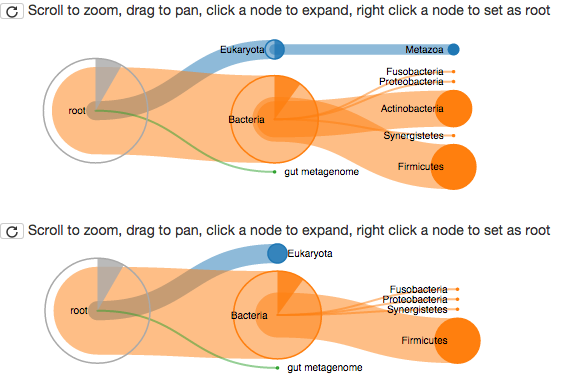
\includegraphics[width=0.7\textwidth]{includes/visexample2}
    \caption{Visualisatie van de HTML-code in \Cref{lst:visexample2}}
    \label{fig:visexample2}
\end{figure}

\subsection{Abstractie: Overschrijven van standaardmethodes}
Met een tweede case study tonen we aan hoe de gebruiker bepaalde functies kan
overschrijven met zijn eigen implementatie.

Indien de gebruiker een grafische zoektocht willen starten naar bepaalde
speciale gevallen in de taxonomie, zoals taxons die rangloos zijn en daarnaast
ook enkele taxons willen invalideren die aan bepaalde voorwaarden voldoen, dan
kan hij de volgende procedure gebruiken. De gebruiker kan van een standaard
JSON-representatie van de boom starten, waarvan hij het \texttt{data}-attribuut
aanvult met twee eigen attributen \texttt{rank} en \texttt{valid\_taxon}. Een
taxon is rangloos wanneer zijn rang gelijk is aan ``no rank'' en een taxon is
\texttt{invalid} wanneer het \texttt{valid\_taxon} attribuut gelijk is aan $0$.
Het JavaScript-gedeelte van de code kan teruggevonden worden in
\Cref{lst:visexample3} op \cpageref{lst:visexample3}.

Eerst definiëren we de twee gewenste functies: een functie die de randkleur van
de node aanpast en een functie die de opvulkleur van de node aanpast. In beide
gevallen geven we ``red'' terug wanneer het \texttt{valid\_taxon}-attribuut van
het \texttt{data}-attribuut op 0 staat. Wanneer de \texttt{rank} gelijk is aan
``no rank'' geven we ``grey'' terug. In alle andere gevallen vallen we telkens
terug op de standaardimplementatie die beschikbaar is via het conventionele
\texttt{Constructor}-attribuut van de \texttt{treeview}-functie. Deze functies
geven dan uiteindelijk mee aan de oproep naar de \texttt{treeview}-methode zodat
die functies de standaardimplementaties overschrijven.

\begin{lstlisting}[caption={JavaScriptgedeelte van de voorbeeldcode ter 
illustratie van 
abstractie van de \texttt{treeview}-visualisatie},label={lst:visexample3}, 
float]
// Eigen implementatie van de nodeStrokeColor functie
var nodeStrokeColor = function(d) {
  if(d.data.valid_taxon !== 1) {
    return "red";
  }
  if (d.data.rank === "no rank") {
    return "gray";
  }
  return $.fn.treeview.Constructor.NODE_STROKE_COLOR(d);
};

// Eigen implementatie van de nodeFill functie
var nodeFillColor = function(d) {
  if(d.data.valid_taxon !== 1) {
    return "red";
  }
  return $.fn.treeview.Constructor.NODE_FILL_COLOR(d);
}

d3.json("../sample-data/hierarchical-taxons-flat.json", 
function(error, data) {
  if (error) return console.warn(error);

  /* Initieert de treeview voor het #d3TreeView element waarbij we de eigen 
  functies meegeven */
  $("#d3TreeView").treeview({
    data: data,
    nodeStrokeColor: nodeStrokeColor,
    nodeFillColor: nodeFillColor,
  });
});
\end{lstlisting}

Het resultaat van \Cref{lst:visexample3} is te zien in 
\Cref{fig:visexample3}. We zien inderdaad dat de nodes die geen rang hebben 
zoals onder meer \texttt{root} en \texttt{cellular organisms}, een 
grijze rand krijgen en dat geïnvalideerde nodes, zoals de volledige tak van de 
``other sequences'', rood opgevuld worden. Bij de overige nodes wordt de 
standaard opvul- en randkleur gebruikt.

\begin{figure}
    \centering
    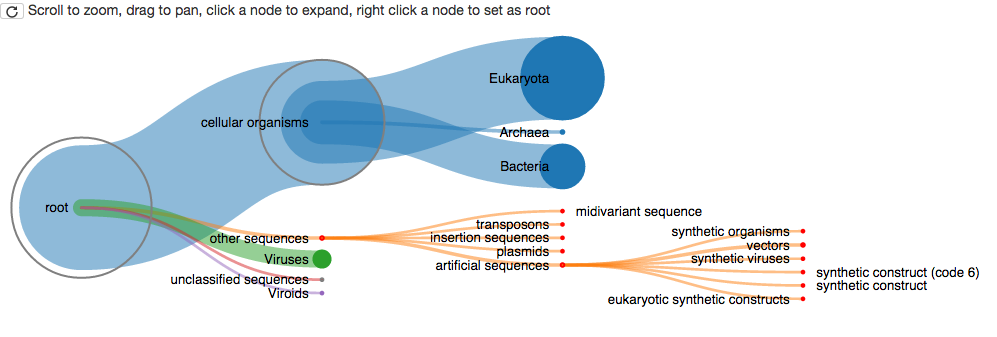
\includegraphics[width=0.9\textwidth]{includes/visexample3}
    \caption{Resultaat van de HTML-code in \Cref{lst:visexample3}}
    \label{fig:visexample3}
\end{figure}

\subsection{Niet-biologische invoerdata}
Zoals in de inleiding vermeld, willen we niet enkel de visualisaties 
specialiseren op biologische data. We kunnen zonder problemen eender welke 
hiërarchische data omvormen tot een JSON-object dat kan gevisualiseerd worden  
in de \texttt{treeview}. Zo kunnen we bijvoorbeeld een opdeling van Europa 
definiëren aan de hand van JSON in \Cref{lst:visexample4} op 
\cpageref{lst:visexample4}. Dit resulteert in de visualisatie in 
\Cref{fig:visexample4} op \cpageref{fig:visexample4}.

\begin{lstlisting}[caption={JSON-representatie van een opdeling van Europa als 
invoer voor de \texttt{treeview}-visualisatie.}, 
label={lst:visexample4}, float]
{
  "id": 1,
  "name": "Europe",
  "data": {
    "count": 100,
    "self_count": 100
  },
  "children": [
    {
      "id": 2,
      "name": "Central Europe",
      "data": {
        "count": 20,
        "self_count": 20,
        "color": "yellow"
      }
    },
    {
      "id": 6,
      "name": "Western Europe",
      "data": {
        "count": 20,
        "self_count": 20,
        "color": "red"
      },
      "children": [
        {
          "id": 7,
          "name": "Belgium",
          "data": {
            "count": 5,
            "self_count": 5
          }
        },
        {
          "id": 8,
          ...
\end{lstlisting}

\begin{figure}
    \centering
    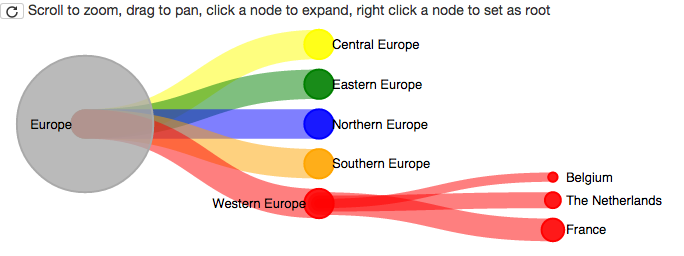
\includegraphics[width=0.9\textwidth]{includes/visexample4}
    \caption{Resultaat van de visualisatie van niet-biologische invoerdata uit 
    \Cref{lst:visexample4}}
    \label{fig:visexample4}
\end{figure}


\section[Optimalisaties aan de bestaande 
\texttt{treeview}-visualisatie]{Optimalisaties aan de bestaande 
\texttt{treeview}-visualisatie%
  \sectionmark{Optimalisaties}}
\sectionmark{Optimalisaties}

Aan de bestaande treeview-visualisatie konden ook nog enkele verbeteringen  
worden doorgevoerd.

Een eerste probleem was dat de huidige code ervoor zorgde dat de opgegeven
hoogte altijd behouden werd. Bij kleine visualisaties was dit geen probleem.
Wanneer er echter een grote hoeveelheid data werd weergegeven, dan zorgde dit 
ervoor dat kleine nodes soms onder grote nodes terechtkwamen. Hierdoor waren 
sommige nodes niet meer aanklikbaar. Dit effect is te zien op 
\Cref{fig:treeviewbefore} 
op \cpageref{fig:treeviewbefore}. De oorzaak hiervan was dat de D3 
\texttt{tree} layout werd ingesteld met een vaste hoogte via
\lstinline|d3.layout.tree().size([height, width])|.

Om dit probleem tegen te gaan heeft D3 een ingebouwde functie, 
\texttt{tree.seperation()}\cite{d3treeseperation:online}. Deze functie zorgt 
ervoor dat een meegegeven functie kan gebruikt worden om de afstand tussen de 
nodes te bepalen. De functie vereist wel dat ook de \texttt{nodeSize} van de 
\texttt{d3.tree} wordt ingesteld. De resulterende code kan worden gevonden in
\autoref{lst:fixseperation} op \autopageref{lst:fixseperation}.
Samengevat wordt de afstand tussen de nodes berekend aan de hand van hun 
nodesize, met enkele pixels extra ruimte ertussen. Wanneer beide nodes niet 
dezelfde ouder hebben, wordt de extra ruimte nog wat uitgebreid zodat er een 
duidelijkere scheiding is tussen groepen kinderen van verschillende oudernodes. 
Het resultaat van deze aanpassing is te zien op \Cref{fig:treeviewafter} op 
\cpageref{fig:treeviewafter}. Alle nodes hebben nu evenveel ruimte 
tussen elkaar en overlappen niet, waardoor alle nodes aanklikbaar blijven.

\begin{lstlisting}[caption=Dynamische schaling van plaats tussen nodes in de 
\texttt{treeview}-visualisatie,label=lst:fixseperation]
tree = d3.layout.tree()
    .nodeSize([2, 10]);
    .separation(function(a, b) {
        var width = (nodeSize(a) + nodeSize(b)),
        distance = width / 2 + 4;
        return (a.parent === b.parent) ? distance : distance + 4;
    });
\end{lstlisting}

\begin{figure}
\centering
\begin{subfigure}{0.42\textwidth}
    \centering
    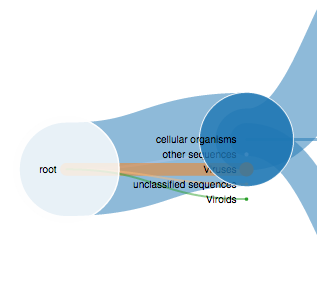
\includegraphics[width=0.9\textwidth]{includes/treeviewbefore}
    \label{fig:treeviewbefore}
\end{subfigure}%
\begin{subfigure}{0.42\textwidth}
    \centering
    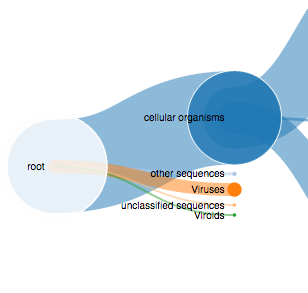
\includegraphics[width=0.9\textwidth]{includes/treeviewafter}
    \label{fig:treeviewafter}
\end{subfigure}
\caption{Voorbeeld van voor (links) en na (rechts) het oplossen van overlappende
nodes van de \texttt{treeview}-visualisatie. Links zien we dat de nodes ``other
sequences'' en ``viruses'' onder node zitten van ``cellular organisms''. Rechts
is dit probleem opgelost: geen enkele node overlapt, waardoor ze aanklikbaar
blijven.} \label{fig:treeviewbeforeandafter}
\end{figure}

Een tweede probleem, ditmaal specifiek toegepast op de metagenomics data, is het
volgende: stel dat we een hiërarchische visualisatie willen weergeven van het
aantal gevonden taxons in een sample data, dan kan dat worden weergegeven op de
\texttt{treeview}-visualisatie waarbij de grootte van nodes overeen komt met het
aantal samples gevonden in die tak van de boom. In
\cref{fig:treeviewarcbefore} op \cpageref{fig:treeviewarcbefore} wordt de
bijhorende visualisatie gemaakt ter analyse van een stoelgangstaal van een mens.
Het is duidelijk te zien dat de grootste aantallen gevonden worden in de tak van
de bacteriën en van de eukaryoten. Wat echter niet meteen zichtbaar is, is het
onderscheid tussen hoeveel peptides worden gemapt op het niveau van de bacteriën
zelf, en hoeveel eigenlijk dieper in die tak worden gevonden. We kunnen aan de
grootte van de nodes inschatten hoeveel dit ongeveer zou kunnen zijn, maar
naarmate een node meer en meer kinderen heeft, wordt dit steeds.

Aangezien de nodes worden voorgesteld door middel van cirkels is het aangewezen
om dit als een taartdiagram aan te duiden met twee delen: het doorzichtige deel
is specifiek voor die tak, maar niet voor de node, terwijl het opgevulde deel
het aantal elementen voorstelt specifiek voor de node.
Door op de node zelf visueel aan te duiden hoeveel peptides specifiek tot op dat
niveau en niet dieper worden gemapt, kunnen we dit proces gemakkelijker maken.

Momenteel worden de nodes in D3 weergegeven door een \texttt{circle} achteraan 
toe te voegen aan de node-objecten. Deze \texttt{circle} krijgt een aantal 
attributen zoals straal, lijndikte, opvullingskleur en lijnkleur. Op dezelfde 
manier dat we een cirkel toevoegen, kunnen we ook een D3 \texttt{arc} 
toevoegen\cite{d3arc:online}. Dit resulteert in de volgende code:

\begin{lstlisting}
// Definieert een arc-scale zodat deze altijd tussen 0 en 2 Pi ligt
arcScale = d3.scale.linear().range([0,2*Math.PI]);

// Definieert een arc-object
var arc = d3.svg.arc()
    .outerRadius(nodeSize)
    .startAngle(0)
    .endAngle(arcSize);

// Voegt de arc toe aan de node wanneer deze wordt upgedatet
nodeUpdate.select("path")
    .duration(duration)
    .attr("d", arc);
\end{lstlisting}

Wanneer een node niet is opengeklapt wordt altijd de volledige node gevuld. Het 
resultaat van die aanpassing is te zien op \Cref{fig:treeviewarcbefore} op 
\cpageref{fig:treeviewarcafter}. De nodes ``organism'', ``Bacteria'' en 
``Eukaryota'' hebben nu allemaal een slice die aangeeft hoeveel peptides er in 
die dataset specifiek op die node gemapt zijn. Dit is in één oogopslag te 
zien, zonder dat het aantal moet worden afgeleid uit de grootte van 
de kinderen.

\begin{figure}
\centering
\begin{subfigure}{0.45\textwidth}
    \centering
    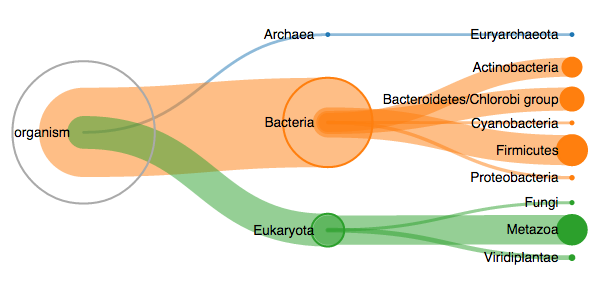
\includegraphics[width=0.95\textwidth]{includes/treeviewnoarc}
    \label{fig:treeviewarcbefore}
\end{subfigure}%
\begin{subfigure}{0.45\textwidth}
    \centering
    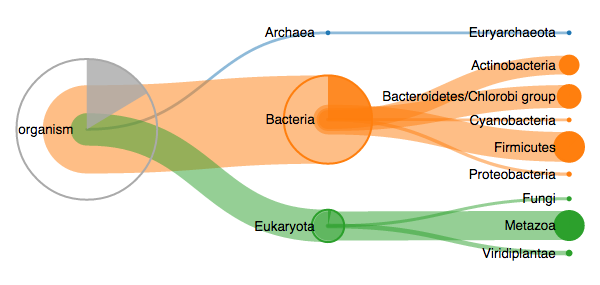
\includegraphics[width=0.95\textwidth]{includes/treeviewarc}
    \label{fig:treeviewarcafter}
\end{subfigure}
\caption{Voorbeeld van voor (links) en na (rechts) het toevoegen van slices in 
de nodes van de \texttt{treeview}-visualisatie. Links is moeilijk in te 
schatten hoeveel procent van de eiwitten op organismeniveau gemapt worden. 
Rechts kunnen we dit wel meteen inschatten aan de hand van de gekleurde slice 
op de node.}
\label{fig:treeviewarc}
\end{figure}

Naast deze twee wijzigingen, werden ook nog enkele gedupliceerde code in 
functies 
ondergebracht, maar dit laten we hier nu buiten beschouwing.

\section{Benchmarking}
We kunnen ons de vraag stellen hoe performant de treeview-visualisatie is en of 
deze 
performant blijft naarmate we meer en meer data toevoegen. Momenteel 
wordt de visualisatie zonder problemen gebruikt om de resultaten van Unipept 
Metaproteomics Analysis Pipeline visueel weer te geven. Wanneer we echter met 
metagenomics data werken is 
deze vaak veel groter dan metaproteomics data, wat misschien mogelijks 
problemen kan opleveren.

De ultieme manier om dit te testen is om de grootst mogelijke dataset in te 
laden voor metagenomics data: de volledige NCBI taxonomie
\cite{ncbitaxonomy:online}.
Deze taxonomie bevat op het moment van schrijven 1.267.511 taxa. Een 
screenshot
van deze visualisatie kan gevonden worden in \Cref{fig:fulltaxy} op
\cpageref{fig:fulltaxy}. Aangezien de visualisatie dynamisch en interactief is,
kan deze ook in zijn geheel bekeken worden op
\url{https://github.ugent.be/pages/unipept/unipept-visualizations/samples/treeview-ncbi-taxonomy.html}.

Vanaf een lokale machine duurt het gemiddeld vier seconden om de visualisatie te
laden. Vanaf de Github Pages is dit ongeveer 51 seconden. Let wel dat deze data
volledig in JavaScript geladen wordt. Dit gebeurt volledig client side wat dus
ook wil zeggen dat alle data eerst gedownload dient te worden,
alvorens de visualisatie kan worden opgezet. De data die in deze visualisatie
geladen wordt, is als platte tekst ongeveer 147 MB groot. Met een connectie van
25 mbit per seconde is van die 51 seconden dus ongeveer 47 seconden download, en
vier seconden effectieve rendering.

Bij dit laatste is het belangrijk dat we een onderscheid maken tussen data die
lokaal geladen wordt en data die via een externe server in de browser geladen 
wordt.
Aangeboden visualisaties op een website zullen hoogstwaarschijnlijk nooit zo
groot zijn als de volledige NCBI taxonomie. Wanneer data van deze omvang wordt
gevisualiseerd, dan zal dit meestal het gevolg zijn van een analyse op een 
lokale
machine, waarbij de data van dezelfde machine afkomstig is en men niet gebonden
is aan een beperkte downloadsnelheid.

\begin{figure}
\centering
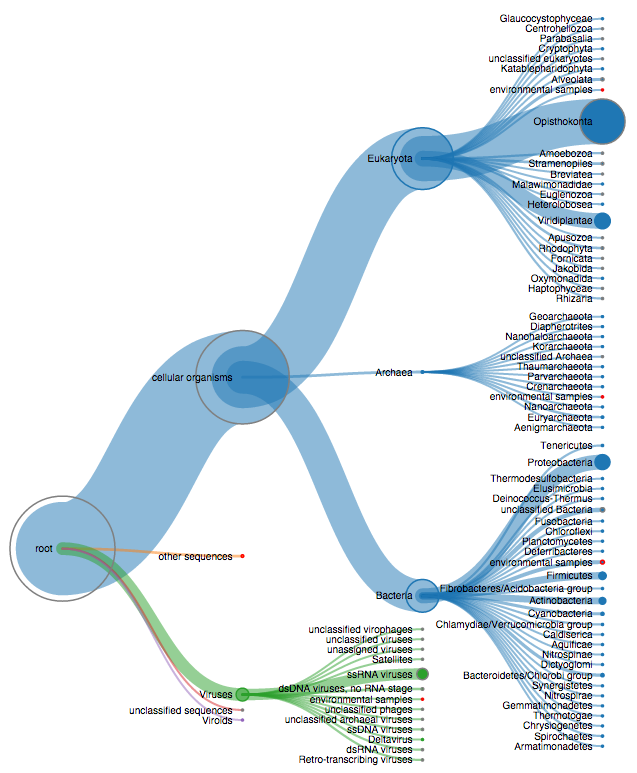
\includegraphics[width=0.9\textwidth]{includes/fulltaxy}
\caption{Screenshot van (een deel van) de volledig NCBI taxonomie 
gevisualiseerd met de \texttt{treeview}-visualisatie.}
\label{fig:fulltaxy}
\end{figure}

Een ander punt is dat de visualisatie ook in alle gevallen responsief dient te 
blijven, ook met grote hoeveelheden data. Aangezien D3 enkel de data toont 
en animeert die zichtbaar is, is dit geen probleem. We hebben ondervonden dat 
zelfs wanneer er heel veel nodes openstaan de 
visualisatie nog steeds responsief blijft.

\section{Conclusie}
De visualisaties zijn zoals die initieel in Unipept ingebed zaten, waren niet 
alleen geschikt om binnen Unipept gebruikt te worden voor de visualisatie en 
analyse van metaproteomische
of metagenomische data, maar kunnen dus ook voor andere doeleinden gebruikt 
worden. Hiervoor kunnen de visualisaties -- zoals overlopen in
\Cref{sec:unipeptvis} -- op dezelfde manier als de
\texttt{treeview}-visualisatie omgevormd worden tot abstracte en modulaire
modules, die dan terug in Unipept kunnen ingeplugd worden. De plugins kunnen
daarnaast ook gebruikt worden om de resultaten van de command-line interface te
visualiseren zonder te steunen op het volledige Unipept-platform en zouden zelfs
kunnen gebruikt worden om niet-biologische data te analyseren.


\section{Toekomstig werk}

In dit hoofdstuk werd als voorbeeld de \texttt{treeview}-visualisatie
geabstraheerd en omgevormd. Zoals echter in de inleiding tot de verschillende
visualisaties in Unipept werd vernoemd zijn er nog meer visualisaties dan enkel
de treeview. Om tot een volwaardig visualisatieframework te komen moeten niet
enkel de andere visualisaties worden omgevormd, maar moeten we het inpluggen van
data ook zo gemakkelijk mogelijk maken voor de gebruiker. Hiervoor zouden we de
Unipept command-line interface kunnen uitbreiden met een parameter die
bijvoorbeeld automatisch het bekomen resultaat visualiseert. Een hele reeks
features die momenteel in Unipept zijn ingebouwd zoals het opslaan van een
visualisatie als afbeelding of het fullscreen bekijken van een visualisatie
zouden moeten worden overgenomen. Het zou ook handig zijn mocht de
visualisatiedata eenvoudig kunnen worden verdeeld onder onderzoekers die aan
hetzelfde project werken.